\documentclass{assignment}
\UsingEnglish
\ProjectInfos*{Intro to Communication System}{EE140}{Fall, 2020}{Assignment 7}{Due time : 10:15, Nov 20, 2020 (Friday)}{陈稼霖}{45875852}
\usepackage{diagbox}
\begin{document}
\begin{prob}[2.1 Coin flip.]
    A fair coin is flipped until the first head occurs. Let $X$ denote the number of flips required.
    \begin{itemize}
        \item[(a)] Find the entropy $H(X)$ in bits. The following expression may be useful:
        \[
            \sum_{n=0}^{\infty}r^n=\frac{1}{1-r},\quad\sum_{n=0}^{\infty}nr^n=\frac{r}{(1-r)^2}.
        \]
        \item[(b)] A random variable $X$ is drawn according to this distribution. Find an "efficient" sequence of yes-no questions of the form, "Is $X$ contained in the set $S$?" Compare $H(X)$ to the expected number of questions required to determine $X$.
    \end{itemize}
\end{prob}
\begin{sol}
    \begin{itemize}
        \item[(a)] The PMF of $X$ is
        \begin{align}
            P(X=n)=\left(\frac{1}{2}\right)^{n-1}\frac{1}{2}=\frac{1}{2^n},\quad n=1,2,3,\cdots
        \end{align}
        The entropy of $X$ in bits is
        \begin{align}
            H(X)=-\sum_{n=1}^{\infty}P(X=n)\log_2P(X=n)=-\sum_{n=1}^{\infty}\frac{1}{2^n}\log_2\frac{1}{2^n}=\sum_{n=1}^{\infty}\frac{n}{2^n}=\frac{\frac{1}{2}}{\left(1-\frac{1}{2}\right)^2}=2\text{ (bits)}.
        \end{align}
        \begin{itemize}
            \item[(b)] We can use Huffman code to represent the possible $X$'s according to the PMF of $X$. That is,
            \begin{align*}
                X=1\rightarrow&1,\\
                X=2\rightarrow&01,\\
                X=3\rightarrow&001,\\
                \cdots&\\
                X=n\rightarrow&\overbrace{00\cdots 0}^{n-1\text{ zeros in total}}1,\\
                \cdots&
            \end{align*}
            Then, we can ask in such way: "Is the first symbol of the code $1$?" If the answer is "Yes", we know that $X=1$. If not, we continue to ask: "Is the second symbol of the code $1$". If the answer is "Yes", then we know that $X=2$. If not, we continue such asking method until the answer is "Yes" and thus we can determine the $X$ represented by the code.\\
            This asking method is equivalent to ask: "Is $X=1$?" "If not, is $X=2$?" "If not, is $X=3$?"......\\
            In such way, the expected number of questions required to determine $X$ is
            \begin{align}
                \frac{1}{2}\times 1+\frac{1}{2}\times\frac{1}{2}\times 2+\frac{1}{2}\times\frac{1}{2}\times\frac{1}{2}\times 3\cdots=\sum_{n=1}^{\infty}\frac{n}{2^n}=2,
            \end{align}
            which equals $H(X)$ in bits.
        \end{itemize}
    \end{itemize}
\end{sol}

\begin{prob}[2.2 Entropy of functions.]
    Let $X$ be a random variable taking on a finite number of values. What is the (general) inequality relation of $H(X)$ and $H(Y)$ if
    \begin{itemize}
        \item[(a)] $Y=2^X$?
        \item[(b)] $Y=\cos X$?
    \end{itemize}
\end{prob}
\begin{sol}
    \begin{itemize}
        \item[(a)] Suppose the set of possible values that $X$ can take on to be $\{x_1,x_2,\cdots,x_N\}$. The entropy of $X$ is
        \begin{align}
            H(X)=-\sum_{n=1}^NP(X=x_n)\log_2P(X=x_n).
        \end{align}
        Since $Y=2^X$ is a one-to-one mapping, the set of the possible values that $Y$ can take on is $\{y_1=2^{x_1},y_2=2^{x_2},\cdots,y_n=2^{x_N}\}$ and the PMF of $Y$ is
        \begin{align}
            P(Y=2^{x_n})=P(X=x_n).
        \end{align}
        The entropy of $Y$ is equal to $X$'s:
        \begin{align}
            H(Y)=-\sum_{n=1}^NP(Y=2^{x_n})\log_2P(Y=2^{x_n})=-\sum_{n=1}^NP(X=x_n)\log_2P(X=x_n)=H(X).
        \end{align}
        \item[(b)] Since $Y=\cos X$ is not necessarily one-to-one, the PMF of $Y$ is
        \begin{align}
            P(Y=y)=\sum_{x\in\{x\vert y=\cos x\}}P(X=x)
        \end{align}
        The entropy of $Y$ is equal to or less than $X$'s:
        \begin{align}
            \notag H(Y)=&-\sum_yP(Y=y)\log_2P(Y=y)\\
            \notag=&-\sum_y\left[\sum_{x\in\{x\vert y=cos x\}}P(X=x)\right]\log_2\left[\sum_{x\in\{x\vert y=\cos x\}} P(X=x)\right]\\
            \notag\leq&-\sum_y\sum_{x\in\{x\vert y=cos x\}}P(X=x)\log_2P(X=x)\\
            =&-\sum_xP(X=x)\log_2P(X=x)=H(X).
        \end{align}
    \end{itemize}
\end{sol}

\begin{prob}[2.4 Entropy of functions of a random variable.]
    Let $X$ be a discrete random variable. Show that the entropy of a function of $X$ is less than or equal to the entropy of $X$ by justifying the following steps:
    \begin{align*}
        H(X,g(X))\overset{\text{(a)}}{=}&H(X)+H(g(X)\vert X)\\
        \overset{\text{(b)}}{=}&H(X);\\
        H(X,g(X))\overset{\text{(c)}}{=}&H(g(X))+H(X\vert g(X))\\
        \overset{\text{(d)}}{\geq}&H(g(X)).
    \end{align*}
    Thus, $H(g(X))\leq H(X)$.
\end{prob}
\begin{pf}
    \begin{itemize}
        \item[(a)] 
        \begin{align}
            \notag H(X,g(X))=&-\sum_{x,y}P(X=x,g(X)=y)\log_2P(X=x,g(X)=y)\\
            \notag=&-\sum_{x,y}P(X=x)P(g(X)=y\vert X=x)\log_2\left[P(X=x)P(g(X)=y\vert X=x)\right]\\
            \notag=&-\sum_{x,y}P(X=x)P(g(X)=y\vert X=x)\log_2P(X=x)\\
            \notag&-\sum_{x,y}P(X=x)P(g(X)=y\vert X=x)\log_2P(g(X)=y\vert X=x)\\
            \notag=&-\sum_xP(X=x)\log_2P(X=x)-\sum_xP(X=x)H(g(X)\vert X=x)\\
            \notag=&H(X)+H(g(X)\vert X).
        \end{align}
        \item[(b)] Once the value of $X$ is given, $g(X)$ is determined, so
        \begin{gather}
            H(g(X)\vert X=x)=0,\\
            \Longrightarrow H(g(X)\vert X)=\sum_xP(X=x)H(g(X)\vert X=x)=0,
        \end{gather}
        and
        \begin{align}
            H(X,g(X))=H(X)+H(g(X)\vert X)=H(X).
        \end{align}
        \item[(c)] 
        \begin{align}
            \notag H(X,g(X))=&-\sum_{x,y}P(X=x,g(X)=y)\log_2P(X=x,g(X)=y)\\
            \notag=&-\sum_{x,y}P(g(X)=y)P(X=x\vert g(X)=y)\log_2\left[P(g(X)=y)P(X=x\vert g(X)=y)\right]\\
            \notag=&-\sum_{x,y}P(g(X)=y)P(X=x\vert g(X)=y)\log_2P(g(X)=y)\\
            \notag&-\sum_{x,y}P(g(X)=y)P(X=x\vert g(X)=y)\log_2P(X=x\vert g(X)=y)\\
            \notag=&-\sum_yP(g(X)=y)\log_2P(g(X)=y)+\sum_yP(g(X)=y)H(X\vert g(X)=y)\\
            \notag=&H(g(X))+H(X\vert g(X)).
        \end{align}
        \item[(d)] Since entropy of any discrete random variable is no less than $0$,
        \begin{align}
            H(X\vert g(X))\geq 0,
        \end{align}
        we have
        \begin{align}
            H(X,g(X))=H(g(X))+H(X\vert g(X))\geq H(g(X)).
        \end{align}
    \end{itemize}
    Using (a)-(d), we can obtain $H(g(X))\leq H(X)$.
\end{pf}

\begin{prob}[2.5 Zero conditional entropy.]
    Show that if $H(Y\vert X)=0$, then $Y$ is a function of $X$ [i.e., for all $x$ with $p(x)>0$, there is only one possible value of $y$ with $p(x,y)>0$].
\end{prob}
\begin{pf}
    The entropy of $Y\vert X$ is
    \begin{align}
        \notag H(Y\vert X)=&-\sum_{x,y}P(X=x,Y=y)\log_2P(Y=y\vert X=x).
    \end{align}
    Since
    \begin{align}
        -P(X=x,Y=y)\log_2P(Y=y\vert X=x)\geq 0,\quad\forall x,y,
    \end{align}
    for given $x_0$ and $y_0$,
    \begin{align}
        \notag H(Y\vert X)\geq&-P(X=x_0,Y=y_0)\log_2P(Y=y_0\vert X=x_0)\\
        =&P(X=x_0)P(Y=y_0\vert X=x_0)\log_2P(Y=y_0\vert X=x_0)\geq 0.
    \end{align}
    If $H(Y\vert X)=0$, then
    \begin{align}
        0\geq-P(X=x_0)P(Y=y_0\vert X=x_0)\log_2P(Y=y_0\vert X=x_0)\geq 0,
    \end{align}
    so there must be
    \begin{align}
        -P(Y=y_0\vert X=x_0)\log_2P(Y=y_0\vert X=x_0)=0,
    \end{align}
    for $P(X=x_0)>0$.
    That is,
    \begin{align}
        P(Y=y_0\vert X=x_0)=0,\text{ or }P(Y=y_0\vert X=x_0)=1,
    \end{align}
    for $P(X=x_0)>0$, which means that for all $x_0$ with $P(X=x_0)>0$, there is only one possible value of $y_0$ with $p(X=x_0,Y=y_0)=p(X=x_0)p(Y=y_0\vert X=x_0)=P(X=x_0)>0$.\\
    Therefore, if $H(Y\vert X)=0$, then $Y$ is a function of $X$.
\end{pf}

\begin{prob}[2.11 Measure of correlation.]
    Let $X_1$ and $X_2$ be identically distributed but not necessarily independent. Let
    \[
        \rho=1-\frac{H(X_2\vert X_1)}{H(X_1)}.
    \]
    \begin{itemize}
        \item[(a)] Show that $\rho=\frac{I(X_1;X_2)}{H(X_1)}$.
        \item[(b)] Show that $0\leq\rho\leq 1$.
        \item[(c)] When is $\rho=0$?
        \item[(d)] When is $\rho=1$?
    \end{itemize}
\end{prob}
\begin{sol}
    \begin{itemize}
        \item[(a)] 
        \begin{align}
            \notag\rho=&1-\frac{H(X_2\vert X_1)}{H(X_1)}\\
            \notag=&\frac{H(X_1)-H(X_2\vert X_1)}{H(X_1)}\\
            \notag&(\text{since }X_1\text{ and }X_2\text{ are identically distributed, }H(X_1)=H(X_2))\\
            \notag=&\frac{H(X_2)-H(X_2\vert X_1)}{H(X_1)}\\
            =&\frac{I(X_1;X_2)}{H(X_1)}.
        \end{align}
        \item[(b)] Since $H(X_2\vert X_1)\geq 0$ and $H(X_1)\geq 0$, we have
        \begin{align}
            \rho=1-\frac{H(X_2\vert X_1)}{H(X_1)}\leq 1.
        \end{align}
        Since $H(X_2)\geq H(X_2\vert X_1)$, we have
        \begin{align}
            \rho=\frac{H(X_2)-H(X_2\vert X_1)}{H(X_1)}\geq 0.
        \end{align}
        \item[(c)] When $X_1$ and $X_2$ are independent, $\rho=0$.
        \begin{proof}
            \begin{align}
                \rho=\frac{I(X_1;X_2)}{H(X_1)}=0\Longleftrightarrow I(X_1;X_2)=0\Longleftrightarrow X_1\text{ and }X_2\text{ are independent}.
            \end{align}
        \end{proof}
        \item[(d)] When $X_1$ and $X_2$ have one-to-one mapping, $\rho=1$.
        \begin{proof}
            \begin{align}
                \rho=1-\frac{H(X_2\vert X_1)}{H(X_1)}=1\Longrightarrow H(X_2\vert X_1)=0\Longleftrightarrow X_2\text{ is a function of }X_1.
            \end{align}
            Accordingly,
            \begin{align}
                \rho=\frac{H(X_1)-H(X_2\vert X_1)}{H(X_2)}=\frac{H(X_2)-H(X_1\vert X_2)}{H(X_2)}=0\Rightarrow H(X_1\vert X_2)=0\Longrightarrow X_1\text{ is a function of }X_2.
            \end{align}
            Therefore, $X_1$ and $X_2$ have one-to-one mapping.
        \end{proof}
    \end{itemize}
\end{sol}

\begin{prob}[2.12 Example of entropy.]
    Let $p(x,y)$ be given by
    \begin{table}[H]
        \centering
        \begin{tabular}{|c|c|c|}
        \hline
        \diagbox{$X$}{$Y$} & $0$ & $1$ \\ \hline
        $0$ & $\frac{1}{3}$ & $\frac{1}{3}$ \\ \hline
        $1$ & $0$ & $\frac{1}{3}$ \\ \hline
        \end{tabular}
    \end{table}
    Find:
    \begin{itemize}
        \item[(a)] $H(X)$, $H(Y)$.
        \item[(b)] $H(X\vert Y)$, $H(Y\vert X)$.
        \item[(c)] $H(X,Y)$.
        \item[(d)] $H(Y)-H(Y\vert X)$.
        \item[(e)] $I(X;Y)$.
        \item[(f)] Draw a Venn diagram for the quantities in parts (a) through $e$.
    \end{itemize}
\end{prob}
\begin{sol}
    \begin{itemize}
        \item[(a)] The PMF of $X$ is
        \begin{align}
            P(X=0)=&P(X=0,Y=0)+P(X=0,Y=1)=\frac{1}{3}+\frac{1}{3}=\frac{2}{3},\\
            P(X=1)=&P(X=1,Y=0)+P(X=1,Y=1)=0+\frac{1}{3}=\frac{1}{3}.
        \end{align}
        The PMF of $Y$ is
        \begin{align}
            P(Y=0)=&P(X=0,Y=0)+P(X=1,Y=0)=\frac{1}{3}+0=\frac{1}{3},\\
            P(Y=1)=&P(X=0,Y=1)+P(X=1,Y=1)=\frac{1}{3}+\frac{1}{3}=\frac{2}{3}.
        \end{align}
        The entropy of $X$ is
        \begin{align}
            H(X)=-P(X=0)\log_2P(X=0)-P(X=1)\log_2P(X=1)=-\frac{2}{3}\log_2\frac{2}{3}-\frac{1}{3}\log_2\frac{1}{3}=0.918\text{ (bits)}.
        \end{align}
        The entropy of $Y$ is
        \begin{align}
            H(Y)=-P(Y=0)\log_2P(Y=0)-P(Y=1)\log_2P(Y=1)=-\frac{1}{3}\log_2\frac{1}{3}-\frac{2}{3}\log_2\frac{2}{3}=0.918\text{ (bits)}.
        \end{align}
        \item[(b)] The conditional PMF of $X\vert Y$ is
        \begin{align}
            P(X=0\vert Y=0)=&1,\\
            P(X=1\vert Y=0)=&0,\\
            P(X=0\vert Y=1)=&\frac{1}{2},\\
            P(X=1\vert Y=1)=&\frac{1}{2}.
        \end{align}
        The conditional PMF of $X\vert Y$ is
        \begin{align}
            P(Y=0\vert X=0)=&\frac{1}{2},\\
            P(Y=1\vert X=0)=&\frac{1}{2},\\
            P(Y=0\vert X=1)=&0,\\
            P(Y=1\vert X=1)=&1.
        \end{align}
        The conditional entropy of $X\vert Y$
        \begin{align}
            \notag H(X\vert Y)=&-P(X=0,Y=0)\log_2P(X=0\vert Y=0)-P(X=1,Y=0)\log_2P(X=1\vert Y=0)\\
            \notag&-P(X=0,Y=1)\log_2P(X=0\vert Y=1)-P(X=1,Y=1)\log_2P(X=1\vert Y=1)\\
            \notag=&-\frac{1}{3}\log_21-0-\frac{1}{3}\log_2\frac{1}{2}-\frac{1}{3}\log_2\frac{1}{2}\\
            =&\frac{2}{3}\text{ (bits)}.
        \end{align}
        The conditional entropy of $Y\vert X$ is
        \begin{align}
            \notag H(Y\vert X)=&-P(X=0,Y=0)\log_2P(Y=0\vert X=0)-P(X=0,Y=1)\log_2P(Y=1\vert X=0)\\
            \notag&-P(X=1,Y=0)\log_2P(Y=0\vert X=1)-P(X=1,Y=1)\log_2P(Y=1\vert X=1)\\
            \notag=&-\frac{1}{3}\log_2\frac{1}{2}-\frac{1}{3}\log_2\frac{1}{2}-0-\frac{1}{3}\log_21\\
            =&\frac{2}{3}\text{ (bits)}.
        \end{align}
        \item[(c)] The joint entropy of $X$ and $Y$ is
        \begin{align}
            \notag H(X,Y)=&-P(X=0,Y=0)\log_2P(X=0,Y=0)-P(X=1,Y=0)\log_2P(X=1,Y=0)\\
            \notag&-P(X=0,Y=1)\log_2P(X=0,Y=1)-P(X=1,Y=1)\log_2P(X=1,Y=1)\\
            \notag=&-\frac{1}{3}\log_2\frac{1}{3}-0-\frac{1}{3}\log_2\frac{1}{3}-\frac{1}{3}\log_2\frac{1}{3}\\
            =&\log_23=1.585\text{ (bits)}.
        \end{align}
        \item[(d)] 
        \begin{align}
            H(Y)-H(Y\vert X)=0.251\text{ (bits)}.
        \end{align}
        \item[(e)] The mutual information of $X$ and $Y$ is
        \begin{align}
            I(X;Y)=H(Y)-H(Y\vert X)=0.251\text{ (bits)}.
        \end{align}
        \item[(f)] As shown in figure \ref{A-7-P-6}.
        \begin{figure}[h]
            \centering
            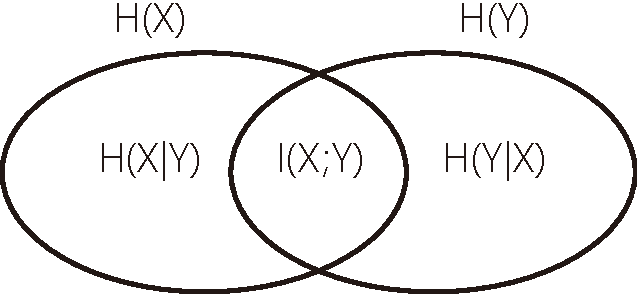
\includegraphics[width=.4\columnwidth]{A-7-P-6.pdf}
            \caption{Venn diagram of $H(X)$, $H(Y)$, $H(X\vert Y)$, $H(Y\vert X)$, $H(X,Y)$ and $I(X;Y)$}
            \label{A-7-P-6}
        \end{figure}
    \end{itemize}
\end{sol}

\begin{prob}[8.1 Diffrential entropy.]
    Evaluate the differential entropy $h(X)=-\int f\ln f$ for the following:
    \begin{itemize}
        \item[(a)] The exponential density, $f(x)=\lambda e^{-\lambda x}$, $x\geq 0$.
        \item[(b)] The Laplace density, $f(x)=\frac{1}{2}\lambda e^{-\lambda\abs{x}}$.
        \item[(c)] The sum of $X_1$ and $X_2$, where $X_1$ and $X_2$ are independent random variables with means $\mu_i$ and variables $\sigma_i^2$, $i=1,2$.
    \end{itemize}
\end{prob}
\begin{sol}
    \begin{itemize}
        \item[(a)] The differential entropy of the exponential density is
        \begin{align}
            \notag h(f)=&-\int_0^{+\infty}\lambda e^{-\lambda x}\ln[\lambda e^{-\lambda x}]\,\mathrm{d}x\\
            \notag=&-\int_0^{+\infty}\lambda e^{-\lambda x}\ln\lambda\,\mathrm{d}x-\int_0^{+\infty}\lambda e^{-\lambda x}(-\lambda x)\,\mathrm{d}x\\
            \notag=&\left.e^{-\lambda x}\ln\lambda\right\rvert_0^{+\infty}-\lambda\int_0^{+\infty}x\,\mathrm{d}(e^{-\lambda x})\\
            \notag=&-\ln\lambda-\left.\lambda xe^{-\lambda x}\right\rvert_0^{+\infty}+\lambda\int_0^{+\infty}e^{-\lambda x}\,\mathrm{d}x\\
            \notag=&1-\ln\lambda\text{ (nats)}\\
            =&\log_2\frac{e}{\lambda}\text{ (bits)}.
        \end{align}
        \item[(b)] The differential entropy of the Laplace density is
        \begin{align}
            \notag h(f)=&-\int_{-\infty}^{+\infty}\frac{1}{2}\lambda e^{-\lambda\abs{x}}\ln\left[\frac{1}{2}\lambda e^{-\lambda\abs{x}}\right]\,\mathrm{d}x\\
            \notag=&\ln 2\int_{-\infty}^{+\infty}\frac{1}{2}\lambda e^{-\lambda\abs{x}}\,\mathrm{d}x-\int_{-\infty}^{+\infty}\frac{1}{2}\lambda e^{-\lambda\abs{x}}\ln[\lambda e^{-\lambda x}]\,\mathrm{d}x\\
            \notag=&\ln 2\text{ (nats)}+\log_2\frac{e}{\lambda}\text{ (bits)}=\log_2\frac{2e}{\lambda}\text{ (bits)}.
        \end{align}
        \item[(c)] $X_1+X_2\sim N(\mu_1+\mu_2,\sigma_1^2+\sigma_2^2)$, thus
        \begin{align}
            h(X_1+X_2)=\frac{1}{2}\log_22\pi e(\sigma_1^2+\sigma_2^2)\text{ (bits)}.
        \end{align}
    \end{itemize}
\end{sol}
\end{document}